\section*{Исходные данные}

\begin{figure}[H]
    \begin{center}
        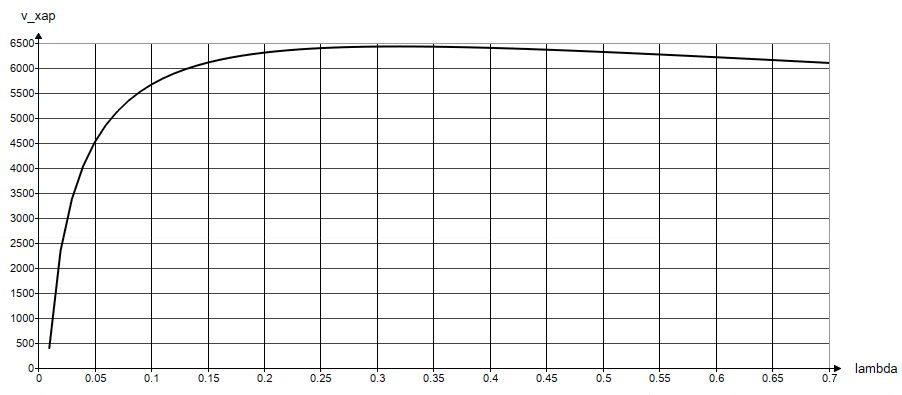
\includegraphics[width = 0.5\linewidth]{pic1.PNG}
        % \caption{Исходные данные}
        \label{pic1}
    \end{center}
\end{figure}

\begin{itemize}
    \item Дальность полета: $L = 3900 \; \t{км}$
    \item Масса полезной нагрузки: $M_{\t{ПГ}} = 2.2 \; \t{т}$
    \item Топливо: АТ + НДМГ
\end{itemize}

В данном задании необходимо:
\begin{itemize}
    \item Провести баллистический расчет
    \item Провести массовый расчет
    \item Провести объемно-габаритный расчет
    \item Построить эскиз вида общего
\end{itemize}

\section*{Решение}
\section{Баллистический расчет}

Найдем дальность баллистического участка:
\begin{equation}
    \label{eq1}
    L_{\t{балл}} = \frac{L}{K_\t{д}} = 3543 \; \t{км}
\end{equation}
где коэффициент дальности $K_\t{д}$ находится по графику (рис. \ref{pic2}).
\begin{figure}[H]
    \begin{center}
        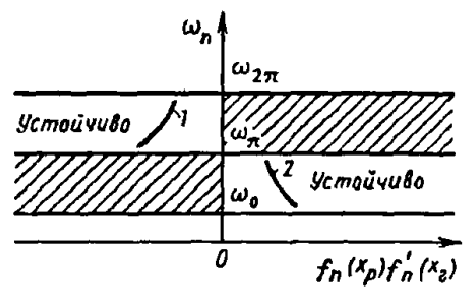
\includegraphics[width = 0.5\linewidth]{pic2.PNG}
        \caption{Зависимость коэффициента дальности $K_\t{д}$ от дальности $L$}
        \label{pic2}
    \end{center}
\end{figure}

Для дальности $L = 3900 \; \t{км}$ он равен $K_\t{д} = 1.1002$.

Тогда угол, на котором разворачивается баллистический участок, равен
\begin{equation}
    \label{eq2}
    \beta = \frac{L_{\t{балл}}}{2R_{\t{З}}} = 15.94^\circ
\end{equation}
где радиус Земли равен $R_\t{З} = 6371 \; \t{км}$.

Определим угол бросания $\phi_A$ по графику (рис. \ref{pic3}):
\begin{figure}[H]
    \begin{center}
        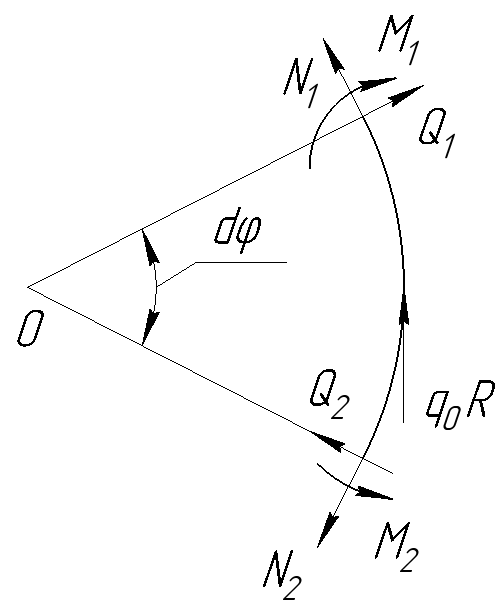
\includegraphics[width = 0.5\linewidth]{pic3.PNG}
        \caption{Зависимость угла бросания $\phi_A$ от угла $\beta$}
        \label{pic3}
    \end{center}
\end{figure}
\begin{equation}
    \label{eq3}
    \phi_A = 37.03^\circ
\end{equation}

Запишем формулу, связывающую угол бросания, относительную скорость и угол $\beta$:
\begin{equation}
    \label{eq4}
    tg \beta = \nu_A \frac{tg \phi_A}{1 - \nu_A + tg^2 \phi_A}
\end{equation}
Получим $\nu_A = 0.431$.

Найдем высоту конца активного участка в первом приближении по зависимости (рис. \ref{pic4}).
\begin{figure}[H]
    \begin{center}
        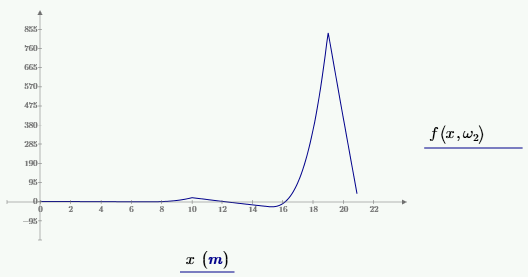
\includegraphics[width = 0.5\linewidth]{pic4.PNG}
        \caption{Зависимость высоты конца активного участка $h_\t{акт}$ от дальности $L$}
        \label{pic4}
    \end{center}
\end{figure}
Для дальности $L = 3900 \; \t{км}$ она равна $h_\t{акт} = 125.6 \; \t{км}$.

Тогда геоцентрический радиус конца активного участка равен
\begin{equation}
    \label{eq5}
    r_A = R_\t{З} + h_A = 6497 \; \t{км}
\end{equation}

Тогда круговая скорость для точки А равна
\begin{equation}
    \label{eq6}
    v_\t{круг} = \sqrt{\frac{\mu}{r_\t{A}}} = 7833 \; \frac{\t{м}}{\t{с}}
\end{equation}

Скорость в конце активного участка равна
\begin{equation}
    \label{eq7}
    v_A = \sqrt{\nu_A \cdot v_\t{круг}^2} = 5142 \; \frac{\t{м}}{\t{с}}
\end{equation}

Проведем расчет второго приближения.

Найдем оптимальный угол бросания
\begin{equation}
    \label{eq8}
    tg\phi_A^\t{опт} = \sqrt{\frac{\nu_A}{2} \cdot \frac{2R_\t{З} - (r_A + R_\t{З}) \nu_A}{R_\t{З} \nu_A + 2(r_A - R_\t{З})}} = 0.719
\end{equation}
\begin{equation}
    \label{eq9}
    \phi_A^\t{опт} = 35.73^\circ
\end{equation}

Уточним параметры, используя выражение
\begin{equation}
    \label{eq10}
    tg \beta = \frac{\nu_A \cdot tg \phi_A^\t{опт}}{1 - \nu_A + tg^2 \phi_A^\t{опт}}
\end{equation}
Откуда получим
\begin{equation}
    \label{eq11}
    \nu_A = 0.431
\end{equation}

Тогда скорость в конце активного участка равна
\begin{equation}
    \label{eq12}
    v_A = \sqrt{\nu_A \cdot v_\t{круг}^2} = 5144 \; \frac{\t{м}}{\t{с}}
\end{equation}

Рассчитаем требуемую характеристическую скорость
\begin{equation}
    \label{eq13}
    v_\t{хар} = v_A + \Sigma \Delta v_i = 6430 \; \frac{\t{м}}{\t{с}}
\end{equation}
где суммарные потери характеристической скорости равны
\begin{equation}
    \label{eq14}
    \Sigma \Delta v_i = 0.25 v_A = 1286 \; \frac{\t{м}}{\t{с}}
\end{equation}

Из формулы Циолковского
\begin{equation}
    \label{eq15}
    v_\t{хар} = - J_\t{п} \ln \mu_\t{к}
\end{equation}
выразим относительную конечную массу ракеты:
\begin{equation}
    \label{eq16}
    \mu_\t{к} = \exp (- \frac{v_\t{хар}}{J_\t{п}}) = 0.134
\end{equation}
где для топливной пары АТ + НДМГ пустотный удельный импульс равен
\begin{equation}
    \label{eq17}
    J_\t{п} = 3200 \; \frac{\t{м}}{\t{с}}
\end{equation}

\section{Массовый расчет}

Запишем весовое уравнение для одноступенчатой ракеты с ЖРД:
\begin{equation}
    \label{eq18}
    G_\t{к} = G_\t{ПГ} + G_\t{ТО} + G_\t{ДУ} + G_\t{пр}
\end{equation}

Разделим это выражение на стартовый вес $G_0$:
\begin{equation}
    \label{eq19}
    \frac{G_\t{к}}{G_0} = \frac{G_\t{ПГ}}{G_0} + \frac{G_\t{ТО}}{G_0} + \frac{G_\t{ДУ}}{G_0} + \frac{G_\t{пр}}{G_0}
\end{equation}

Заменим слагаемые на коэффициенты:
\begin{equation}
    \label{eq20}
    \mu_\t{к} = \mu_\t{ПГ} + a_\t{ТО} (1 - \mu_\t{к}) + \frac{\gamma_\t{ДУ}}{\nu_0} + \mu_\t{пр}
\end{equation}
\begin{equation}
    \label{eq21}
    \frac{G_\t{ТО}}{G_0} = a_\t{ТО} \frac{G_\t{Т}}{G_0} = a_\t{ТО} \frac{G_0 - G_\t{к}}{G_0} = a_\t{ТО} (1 - \mu_\t{к})
\end{equation}
где $a_\t{ТО} = \displaystyle \frac{G_\t{ТО}}{G_\t{Т}}$ --- весовой коэффициент топливного отсека.
\begin{equation}
    \label{eq22}
    \frac{G_\t{ДУ}}{G_0} = \gamma_\t{ДУ} \frac{P_0}{G_0} = \frac{\gamma_\t{ДУ}}{\nu_0} \frac{G_0}{G_0} = \frac{\gamma_\t{ДУ}}{\nu_0}
\end{equation}
где $\gamma_\t{ДУ} = \displaystyle \frac{G_\t{ДУ}}{P_0}$ --- весовой коэффициент двигательной установки, $\nu_0 = \displaystyle \frac{G_0}{P_0}$ --- стартовая нагрузка на тягу.

Из уравнения (\ref{eq20}) получим:
\begin{equation}
    \label{eq23}
    \mu_\t{ПГ} = \mu_\t{к} (1 + a_\t{ТО}) - a_\t{ТО} - \frac{\gamma_\t{ДУ}}{\nu_0} - \mu_\t{пр}
\end{equation}
где $\mu_\t{ПГ} = \displaystyle \frac{M_\t{ПГ}}{M_0}$.

Найдем зависимости весовых коэффициентов от стартовой массы по эмпирическим зависимостям. Для топливной пары АТ + НДМГ они имеют вид:
\begin{equation}
    \label{eq24}
    a_\t{ТО} = 0.033 (1 + 0.5 \exp(-0.014M_\t{Т}))
\end{equation}
\begin{equation}
    \label{eq25}
    \gamma_\t{ДУ} = 0.012 (1 + 1.0 \exp(-0.0009 P_\t{п}))
\end{equation}
\begin{equation}
    \label{eq26}
    \mu_\t{пр} = 0.013 (1 + 0.59 \exp(-0.0048 M_0)) + \frac{0.25}{M_0}
\end{equation}

Зависимость топлива от стартовой массы:
\begin{equation}
    \label{eq27}
    M_\t{Т} = M_0 (1 - \mu_\t{к})
\end{equation}

Расчитаем время работы ДУ:
\begin{equation}
    \label{eq28}
    t_\t{к} = \frac{J_\t{п} \nu_0 (1 - \mu_\t{к})}{k_\t{п} g_0} = 147.373 \; \t{с}
\end{equation}
где $k_\t{п} = 1.15$ --- коэффициент тяги в пустоте, $\nu_0 = 0.6$ --- стартовая нагрузка на тягу.

Секундный массовый расход равен
\begin{equation}
    \label{eq29}
    \dot{m} = \frac{M_\t{Т}}{t_\t{к}} = \frac{M_0 (1 - \mu_\t{к})}{t_\t{к}}
\end{equation}

Тогда пустотная тяга равна
\begin{equation}
    \label{eq30}
    P_\t{п} = \dot{m} J_\t{п} = \frac{M_0 (1 - \mu_\t{к})}{t_\t{к}} J_\t{п}
\end{equation}

Получим зависимость всех весовых коэффициентов от стартовой массы. Тогда весовое уравнение (\ref{eq23}) примет вид
\begin{equation}
    \label{eq31}
    M_0 = \frac{M_\t{ПГ}}{\displaystyle \mu_\t{к}(1 + a_\t{ТО}(M_0)) - a_\t{ТО}(M_0) - \frac{\gamma_\t{ДУ}(M_0)}{\nu_0} - \mu_\t{пр}(M_0)}
\end{equation}

Решая это уравнение, получим
\begin{equation}
    \label{eq32}
    M_0 = 49.142 \; \t{т}
\end{equation}

Найдем составляющие массы ракеты:
\begin{itemize}
    \item Масса топлива
    \begin{equation}
        \label{eq33}
        M_\t{Т} = M_0 (1 - \mu_\t{к}) = 42.553 \; \t{т}
    \end{equation}
    \item Масса горючего:
    \begin{equation}
        \label{eq34}
        M_\t{Г} = \frac{M_\t{Т}}{1 + k_M} = 11.198 \; \t{т}
    \end{equation}
    где $k_M = 2.8$ --- коэффициент избытка окислителя для топливной пары АТ + НДМГ.
    \item Масса окислителя:
    \begin{equation}
        \label{eq35}
        M_\t{ОК} = k_M M_\t{Г} = 31.355 \; \t{т}
    \end{equation}
    \item Масса топливного отсека:
    \begin{equation}
        \label{eq36}
        M_\t{ТО} = a_\t{ТО} M_\t{Т} = 1.791
    \end{equation}
    \item Масса двигательной установки:
    \begin{equation}
        \label{eq37}
        M_\t{ДУ} = \frac{\gamma_\t{ДУ}}{\nu_0} M_0 = 1.411 \; \t{т}
    \end{equation}
    \item Прочая масса:
    \begin{equation}
        \label{eq38}
        M_\t{пр} = \mu_\t{пр} M_0 = 1.187 \; \t{т}
    \end{equation}
\end{itemize}

Выполним проверку:
\begin{equation}
    \label{eq39}
    \begin{split}
        & M_\t{ПГ} + M_\t{Г} + M_\t{ОК} +  M_\t{ТО} + M_\t{ДУ} +M_\t{пр} = 
        \\
        & = 2.2 + 11.198 + 31.355 + 1.791 + 1.411 + 1.187 = 49.142 \; \t{т} = M_0
    \end{split}
\end{equation}

\section{Объемно-габаритный расчет}

Зададимся диаметром ракеты таким образом, чтобы ее удлинение $\displaystyle \lambda = \frac{L}{d}$ было в пределах $\lambda = 8 \dots 12$. Выберем $d = 2$ м.

Будем применять схему с межбаковым отсеком. Примем его длину, равную
\begin{equation}
    \label{eq40}
    L_\t{меж} = 0.1d = 0.2 \; \t{м}
\end{equation}

\subsection{Расчет тоннельной трубы}

Найдем расход окислителя:
\begin{equation}
    \label{eq41}
    \dot{m}_\t{ОК} = \dot{m} \frac{k_M}{1 + k_M} = 212.761 \; \frac{\t{кг}}{\t{с}}
\end{equation}

Тогда диаметр тоннельной трубы равен
\begin{equation}
    \label{eq42}
    d_\t{тр} = \sqrt{\frac{\dot{m}_\t{ОК}}{\frac{\pi}{4}v \rho_\t{ОК}}} = 0.25 \; \t{м}
\end{equation}
где $\displaystyle v = 3 \; \frac{\t{м}}{\t{с}}$ --- скорость движения окислителя по трубе, $\displaystyle \rho_\t{ОК} = 1440 \; \frac{\t{кг}}{\t{м}^3}$ --- плотность окислителя.

Тогда диаметр магистральной трубы равен
\begin{equation}
    \label{eq43}
    d_\t{тон} = d_\t{тр} + 0.06 \; \t{м} = 0.31 \; \t{м}
\end{equation}

\subsection{Расчет баков}

Объем окислителя:
\begin{equation}
    \label{eq44}
    V_\t{ОК} = \frac{M_\t{ОК}}{\rho_\t{ОК}} = 21.774 \; \t{м}^3
\end{equation}

Объем горючего:
\begin{equation}
    \label{eq45}
    V_\t{Г} = \frac{M_\t{Г}}{\rho_\t{Г}} = 14.175 \; \t{м}^3
\end{equation}
где $\displaystyle \rho_\t{Г} = 790 \frac{\t{кг}}{\t{м}^3}$ --- плотность горючего.

Расчитаем объем баков с запасом:
\begin{equation}
    \label{eq46}
    V_\t{БО} = 1.1 V_\t{ОК} = 23.952 \; \t{м}^3
\end{equation}
\begin{equation}
    \label{eq47}
    V_\t{БГ} = 1.1 V_\t{Г} = 15.593 \; \t{м}^3
\end{equation}

Расчитаем вылет баков:
\begin{equation}
    \label{eq48}
    h = 0.25d = 0.5 \; \t{м}
\end{equation}

Найдем радиус днищ баков:
\begin{equation}
    \label{eq49}
    R_\t{дн} = 1.25 \frac{d}{2} = 1.25 \; \t{м}
\end{equation}

Тогда объем сегмента днища равен
\begin{equation}
    \label{eq50}
    V_\t{дн} = \frac{1}{3} \pi h^2 (3R_\t{дн} - h) = 0.851 \; \t{м}^3
\end{equation}

Объем цилиндрической части бака окислителя равен
\begin{equation}
    \label{eq51}
    L_\t{ЦО} = V_\t{БО} - 2V_\t{дн} = 22.25 \; \t{м}^3
\end{equation}

Тогда длина цилиндрической части бака окислителя равна
\begin{equation}
    \label{eq52}
    L_\t{ЦО} = \frac{4V_\t{ЦО}}{\pi d^2} = 7.082 \; \t{м}
\end{equation}

Объем цилиндрической части бака горючего равен
\begin{equation}
    \label{eq53}
    V_\t{ЦГ} = V_\t{БГ} - 2(V_\t{дн} - \frac{\pi d_\t{тон}^2}{4}h) = 13.967 \; \t{м}^3
\end{equation}

Тогда длина цилиндрической части бака горючего равна
\begin{equation}
    \label{eq54}
    L_\t{ЦГ} = \frac{V_\t{ЦГ}}{\displaystyle \frac{\pi}{4} (d^2 - d_\t{тон}^2)} = 4.555 \; \t{м}
\end{equation}

\subsection{Расчет приборного отсека}

Введем следующее допущение:
\begin{equation}
    \label{eq55}
    M_\t{ПО} = \frac{M_\t{пр}}{2} = 593.282 \; \t{кг}
\end{equation}

Тогда объем приборного отсека равен
\begin{equation}
    \label{eq56}
    V_\t{ПО} = \frac{M_\t{ПО}}{\rho_\t{ПО}} = 1.825 \; \t{м}^3
\end{equation}
где $\displaystyle \rho_\t{ПО} = 325 \; \frac{\t{кг}}{\t{м}^3}$ --- принятая плотность приборного отсека.

Тогда длина приборного отсека равна
\begin{equation}
    \label{eq57}
    L_\t{ПО} = \frac{4 V_\t{ПО}}{\pi d^2} = 0.581 \; \t{м}
\end{equation}

\subsection{Расчет головной части}

Зададимся углом раскрытия головной части, равным $40^\circ$. Тогда длина головной части равна
\begin{equation}
    \label{eq58}
    L_\t{ГЧ} = \frac{d}{2 tg 20^\circ} = 2.747 \; \t{м}
\end{equation}

Тогда объем головной части равен
\begin{equation}
    \label{eq59}
    V_\t{ГЧ} = \frac{1}{3} \frac{\pi d^2}{4} L_\t{ГЧ} = 2.877 \; \t{м}^3
\end{equation}

\subsection{Расчет хвостового отсека}

Для упрощения расчетов примем двигатель ракеты однокамерным.

Для топливной пары АТ + НДМГ расходный комплекс равен
\begin{equation}
    \label{eq59.1}
    \beta_\t{Т} = 170 \; \t{с} = 1668 \; \frac{\t{м}}{\t{с}}
\end{equation}

Давление в камере сгорания примем равным
\begin{equation}
    \label{eq59.2}
    p_\t{к} = 10 \; \t{МПа}
\end{equation}

Давление на срезе сопла примем равным
\begin{equation}
    \label{eq59.3}
    p_a = 0.07 \; \t{МПа}
\end{equation}

Показатель процесса расширения для топливной пары равен
\begin{equation}
    \label{eq59.4}
    n = 1.2
\end{equation}

Расчитаем площадь критического сечения:
\begin{equation}
    \label{eq59.4.1}
    S_\t{кр} = \beta_\t{Т} \frac{P_\t{п}}{p_\t{к} J_\t{п}} = 0.048 \; \t{м}^2
\end{equation}

Диаметр критического сечения равен
\begin{equation}
    \label{eq59.4.2}
    d_\t{кр} = \sqrt{\frac{4 S_\t{кр}}{\pi}} = 0.248 \; \t{м}
\end{equation}

Радиус критического сечения равен
\begin{equation}
    \label{eq59.4.3}
    r_\t{кр} = \frac{d_\t{кр}}{2} = 0.124 \; \t{м}
\end{equation}

Тогда площадь выходного сечения сопла равна
\begin{equation}
    \label{eq59.5}
    S_\t{a} = S_\t{кр} \left( \frac{ \displaystyle \frac{n - 1}{2} \left( \frac{2}{n + 1} \right)^{\frac{n + 1}{n - 1}}}{ \displaystyle \left( \frac{p_a}{p_\t{к}} \right)^\frac{2}{n} - \left( \frac{p_a}{p_\t{к}} \right)^{\frac{n + 1}{n}}} \right) = 0.743 \; \t{м}^2
\end{equation}

Тогда диаметр выходного сечения равен
\begin{equation}
    \label{eq59.6}
    d_a = \sqrt{\frac{4 S_a}{\pi}} = 0.973 \; \t{м}
\end{equation}

Радиус выходного сечения равен
\begin{equation}
    \label{eq59.7}
    r_a = \frac{d_a}{2} = 0.486 \; \t{м}
\end{equation}

Проведем расчет закритической части сопла. В качестве первого приближения рассмотрим коническое сопло. Угол раскрытия сопла примем равным $2\beta = 40^\circ$.

Тогда длина этого сопла равна
\begin{equation}
    \label{eq59.8}
    l_\t{К} = \frac{r_a - r_\t{кр}}{tg \beta} = 0.996 \; \t{м}
\end{equation}

В качестве второго приближения примем параболический профиль сопла. Длина его закритической части равна
\begin{equation}
    \label{eq59.9}
    l_\t{закр} = 0.8 l_\t{К} = 0.797 \; \t{м}
\end{equation}

Рассчитаем докритическую часть сопла. Диаметр камеры примем равным
\begin{equation}
    \label{eq59.10}
    d_\t{кам} = 2 d_\t{кр} = 0.495 \; \t{м}
\end{equation}

Тогда радиус камеры сгорания равен
\begin{equation}
    \label{eq59.11}
    r_\t{кам} = \frac{d_\t{кам}}{2} = 0.248 \; \t{м}
\end{equation}

Длину камеры сгорания примем равной
\begin{equation}
    \label{eq59.12}
    l_\t{кам} = 3 d_\t{кр} = 0.743 \; \t{м}
\end{equation}

Примем угол сужения докритической части равным $2 \beta_\t{докр} = 90^\circ$.

Тогда длина докритической части сопла равна
\begin{equation}
    \label{eq59.13}
    l_\t{докр} = \frac{r_\t{кам} - r_\t{кр}}{tg \beta_\t{докр}} = 0.124 \; \t{м}
\end{equation}

Длина сопла равна
\begin{equation}
    \label{eq59.14}
    l_\t{С} = l_\t{докр} + l_\t{закр} = 0.921 \; \t{м}
\end{equation}

Длину двигательной установки примем равной
\begin{equation}
    \label{eq59.15}
    L_\t{ДУ} = 2 l_\t{С} = 1.842 \; \t{м}
\end{equation}

Длину хвостового отсека примем равной длине двигательной установки: 
\begin{equation}
    \label{eq59.16}
    L_\t{ХО} = L_\t{ДУ} = 1.842 \; \t{м}
\end{equation}

\subsection{Расчет длины ракеты}

Расчитаем полную длину ракеты:
\begin{equation}
    \label{eq63}
    L = L_\t{ГЧ} + L_\t{ПО} + L_\t{ЦО} + L_\t{меж} + L_\t{ЦГ} + 4h + L_\t{ХО} = 19.007 \; \t{м}
\end{equation}

Расчитаем удлинение ракеты:
\begin{equation}
    \label{eq64}
    \lambda = \frac{L}{d} = 9.504
\end{equation}
Данное значение находится в допустимых пределах.